\chapter{Introduction}
For the past 50 years, the quest for discovering the cosmos has led to a large array of advances in optics based technology. To overcome the challenges of imaging objects far away and at wavelengths way beyond the capabilities of the human eye, scientists and engineers have come up with ingenious solutions. Specifically, when it comes to imaging and detection in the X-ray energy range ($\sim$0.1-500 keV), whole new obstacles had to be overcome.

The first problem was the inability of X-rays to penetrate Earth's atmosphere, which necessitated detectors to be placed on baloons, sounding rockets or in orbit around earth. That gave rise to a drive for weight saving, miniturization and power conservation.

The next problem that became apparent was the inability of X-rays to be reflected in a mirror in contrast to ground based or orbiting optical telescopes such as Hubble. The high energy of X-rays means that the refractory index of a material become less than unity, so instead of being reflected, the photons are absorbed. However, there is a workaround: The X-ray photons can be reflected at very small grazing angles, e.g. a 10 keV photon can be reflected at up to $\sim$0.5 degrees from a gold surface with almost 100\% intensity. Luckily, the gold is not strickly necessary as any high electron density material will do (anything with a high Z number in the periodic table). Then how can we make an optic that reflects at such low grazing angles, but still has a big collecting area, and preferably also focuses like a parabolic mirror? The answer came from nested shells of concentric mirrors all angled\footnote{It is important to consider that in astrophysical observersations, the photons coming from a distant object are described as completely collimated or in other words: Their trajectories are parralel so all arrive at the optic with the exact same normal angle.} to reflect incoming X-rays to the same spot. Using two sets of mirrors, the first with a parabolic shape and the second with a hyperbolic shape will make it possible to fit the optic in a spacecraft that will fit on a rocket. The design is called a Wolter I type optic\cite{Wolter:1952gt,Wolter:1952ih} (named after the inventor) and specifically addresses the needs for a grazing angle focusing telescope.

Then a new problem comes to light: As the energy of the X-ray photon increases, the grazing angle at which we see reflection from a gold surface decreases dramatically. That leaves us with two options, either increase the length of the optic with extendable masts (costly and technically difficult), or somehow improve the reflecting surface. Looking at the properties of X-rays it was seen that it is possible for an X-ray photon to reflect from the lattice plane of a crystal. Specifically, the photon saw the change in electron density from between the lattice planes to a lattice plane like a surface.\footnote{The reverse argument is more correct. Photons reacting to a surface are just photons reacting to a change in electron density.} Additionally, the photons achieve constructive interference at certain angles related to the photon wavelength and lattice spacing known as the Bragg condition\footnote{$n\lambda=2d\sin(\theta)$ with $\lambda$ being the wavelength, $d$ the lattice spacing and $\theta$ the angle}. So how to take advantage of those X-ray properties? Using lattices means using perfect crystals and shaping them into a Wolter I type optic, both of which creates all new problems\footnote{Using perfect crystals for X-ray and Gamma-ray instrumentation are being investigated and are called Laue lenses\cite{Lund:1992kc,Barriere:2014dj,Barriere:2009cm}.}. Instead the attention was turned to thin film coatings. Advances in technology made it possible to deposit extremely thin and very uniform coatings with a wide variety of materials. By applying a multilayer coating of interchanging materials with low electron density and high electron density, a pseudo crystal can be created. The thickness of each layer can be determined precisely, so in accordance with the Bragg condition the thickness can be designed to reflect at a given angle and photon energy. The constructive interference of the Bragg condition is however a drawback when it comes to astrophysical observations, as only a small bandwidth of photons will be reflected. To overcome that problem, a multilayer with hundreds of layers and film thicknesses that varied from top to bottom was developed. These coatings are called graded-d multilayers and was used for the first time in an astrophysical observatory in the balloon mission HEFT\cite{Koglin:2004tr,Madsen:2003te,Jensen:2002tf}. The successor of HEFT was NuSTAR\cite{Harrison:2013wl,Harrison:2010gu,Harrison:2005wa} that also used power-law graded multilayer coatings on slumped glass substrates\cite{Christensen:2011wg,Brejnholt2012} and was launched in 2012. NuSTAR has from 2012 to 2014 been the NASA mission with the second most published papers from the observations. A short description of NuSTAR can be found in section \ref{sec:nustar}.

{\bf In this thesis is described work done from 2011 to 2014 on coating developments for the European ATHENA mission, the design, production, and installation of an X-ray telescope for the CAST experiment at CERN, and the design of an X-ray telescope for IAXO, the proposed successor to CAST. All of these instruments are Wolter I style X-ray telescopes that function at grazing angles and in an energy band in the very low end compared to NuSTAR, right in the region where there is only a limited benefit from using multilayers compared to single or double layer coatings. }

Chapter \ref{chap:coating_facility} is a description of the coating facility and X-ray measurement setup at DTU Space. A complete overhaul was done to the control software of the coating facility, which is described in detail.

For the coating developments for ATHENA (chapter \ref{chap:athena_coatings}), the main goal was to find coatings that are stable and well-performing. Coatings that will behave well even after being launched by a rocket and drifting around a Lagrange point for 10+ years. At the same time the coatings should be able to reflect well enough to give ATHENA the largest effective area of any X-ray telescope. A new optics technology was developed by ESA leveraged by advances in the semiconductor industry, but require specific processes that would ruin pure carbon coatings, an element used in the NuSTAR coatings. The final problem was finding a way to coat the 300,000 mirrors required for the mission in the 2 years allocated by ESA for mirror production and coating.

The CAST helioscope looks for the hypothetical axion particle, a possible solution to the CP violation problem in particle physics and a candidate for Dark Matter. Using a strong magnetic field to convert axion particles to X-ray photons, CAST is the most comprehensive experiment for detecting axions to date. In order to improve the sensibility of the helioscope, an X-ray telescope was needed to focus photons converted from axions into a small detector. In chapter \ref{chap:cast_xrt} the reader can find a description on all of the work done on an X-ray telescope for CAST.

A proposed successor to the CAST experiment is the International AXion Observatory (IAXO), which is described in chapter \ref{chap:iaxo}, the paper \emph{X-ray optics for axion helioscopes} in appendix \ref{pap:axion_spie}, and the paper \emph{Conceptual design of the International Axion Observatory (IAXO)} of which a relevant part is found in appendix \ref{pap:iaxo_concept}. IAXO is based on the same principle of the CAST helioscope, a superconducting magnet applies a magnetic field to convert axions into X-ray photons. The photons are collected by X-ray telescopes and focused into detectors. Numerous improvements of IAXO over CAST makes the sensitivity more than five orders of magnitude better, making it possible to reach the axion-photon coupling range at which most axions models predict the hypothetical particle will be found.

\section{Coatings for X-ray telescopes}
To focus X-rays in space- or balloon-based telescopes, an array of mirrors with specific coatings is required. When focusing photons in the UV spectrum and longer wavelengths up beyond radio waves, the mirror can be a parabola, since the refractive index deviates from that of unity considerably for longer wavelengths. In the X-ray case however, the refractive index deviation from unity is in the order of $-10^{-5}$, which means that from ambient (vacuum/air, $n=1$) to matter, the direction of the photon is changed very little. In a single lens, the focal length is in the range of 100m. Using a regular lens to focus would require a material with as high a deviation from unity as possible, which means denser materials that results in more absorption. So, normal incidence parabolic focusing and regular refractive focusing are not feasible solutions for focusing X-rays. Instead, grazing incidence reflection is used, since below a very low critical angle $\theta_c$, X-rays will experience total external reflection on a surface\cite{AlsNielsen:2001vt}. $\theta_c$ is connected to the density of the surface material by
\begin{eqnarray}
	\theta_c = \sqrt{2\delta}
\end{eqnarray}
with
\begin{eqnarray}
	\delta = \frac{2\pi \rho_A f^0 (0) r_0}{k^2}
\end{eqnarray}

where $\rho_A f^0 (0)=\rho$ is the electron density of the material. The critical angle can therefore be changed by using a heavier material as a mirror. Recent X-ray missions such as Chandra from NASA and XMM from ESA utilizes mirrors coated with gold to increase $\theta_c$ and decrease the focal length.

% The focal length is still too long to be practical in a space-based telescope, so by letting the incoming photons reflect at low grazing angle on first a parabolic mirror and then a hyperbolic mirror (see figure \ref{fig:doublereflected}), the focal length for gold plated mirrors comes down to a reasonable length (10 m for NuStar and Chandra). The mirrors are mounted in concentric circles with a difference in radius between each layer so that entire mirror length will be used at the angle of incidence, but not more so the mirror rings can be packed as close together as possible.
%
% \begin{figure}[!ht] % double reflected
% 	\centering
% 		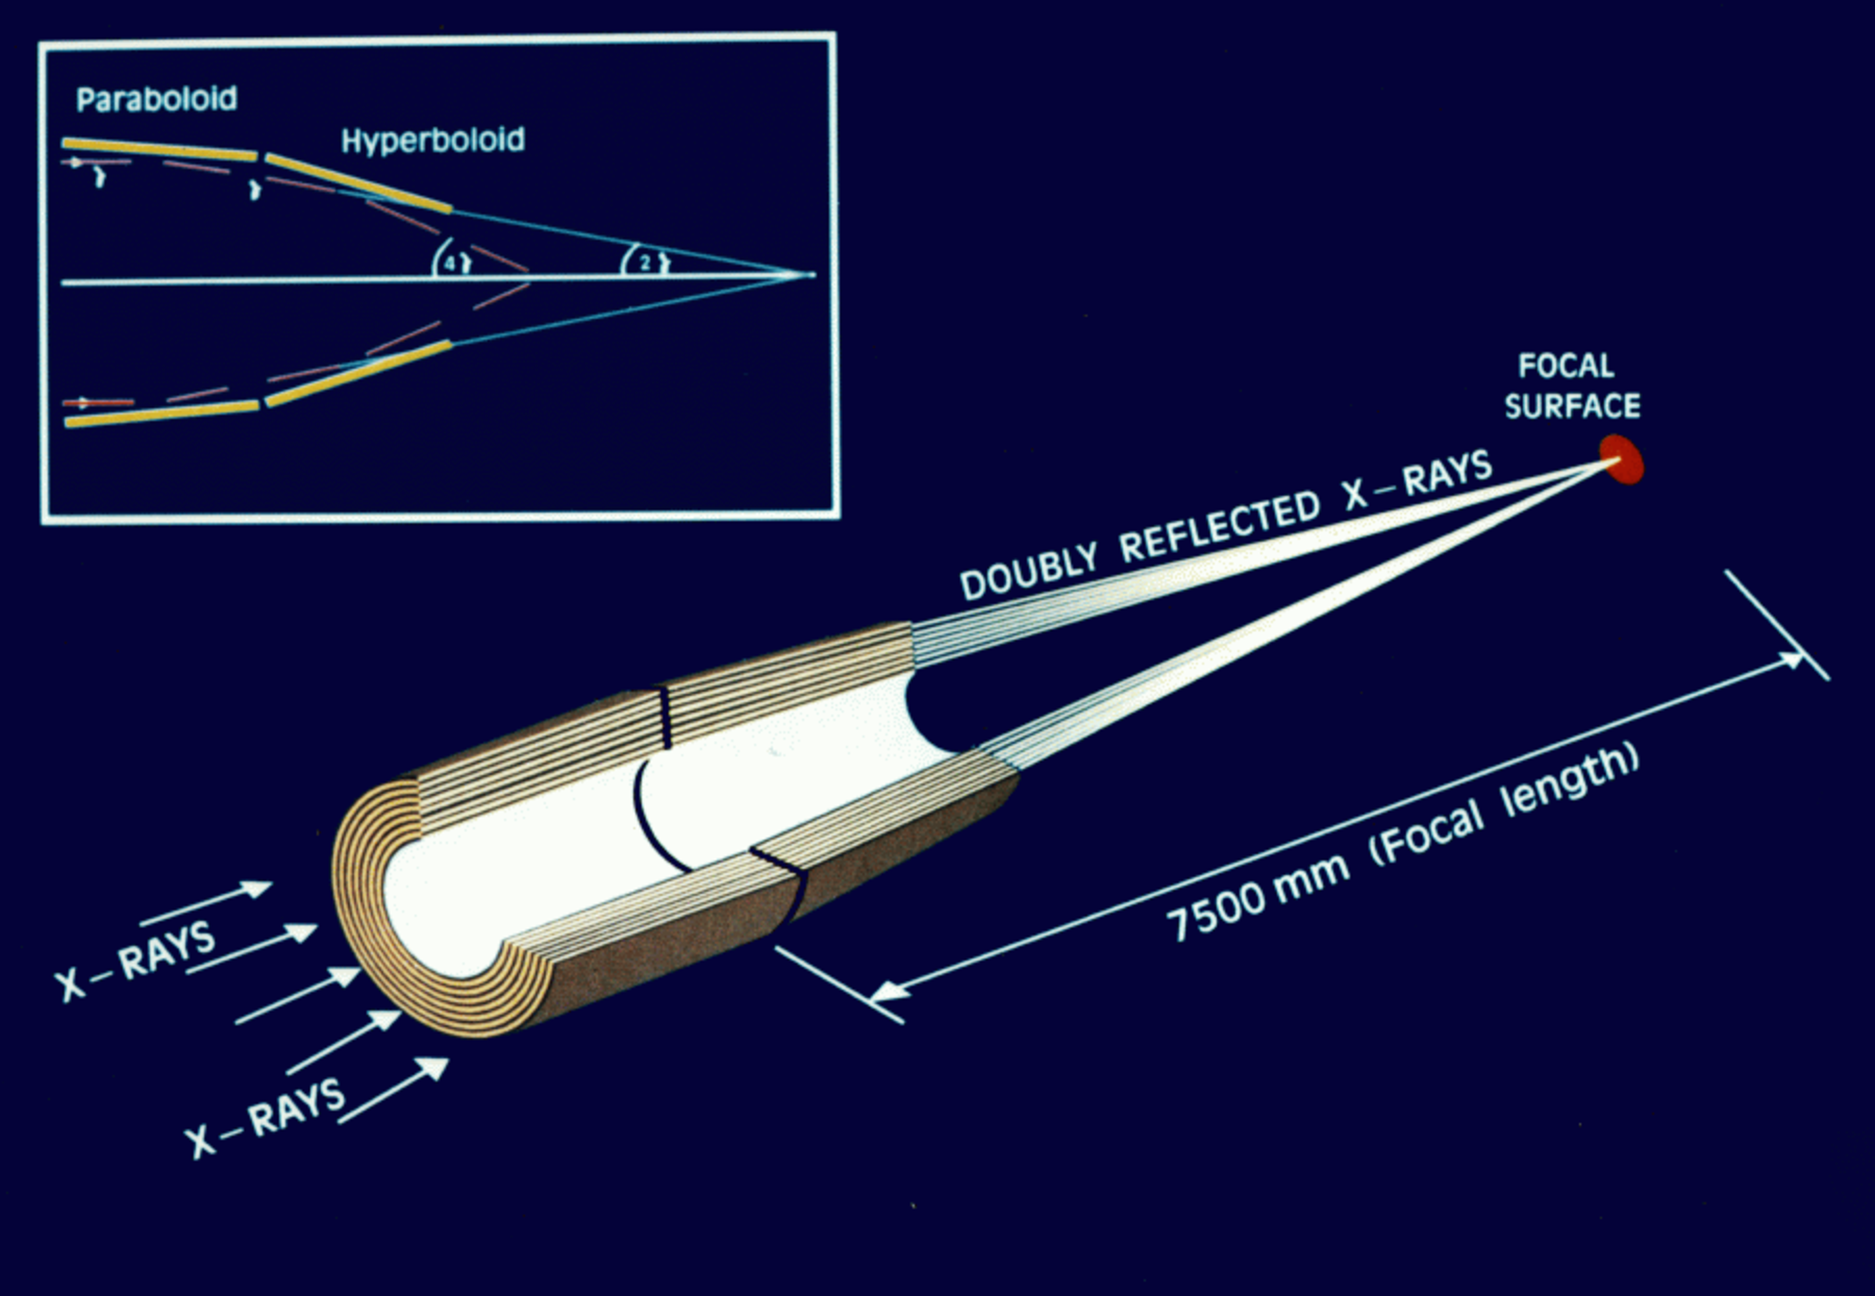
\includegraphics[height=3in]{figures/introduction/xmm.pdf}
% 	\caption{\footnotesize Principle of X-rays focused by double reflection. The incoming photons first hit the parabolic mirror array, and to shorten the focal length, the photons then hit a hyperbolic mirror array. The focal length in this image applies to ESA's XMM telescope. From \url{xmm.esa.int} .}
% 	\label{fig:doublereflected}
% \end{figure}
The mirrors coated with a single high density material have the drawback that they cannot effectively provide reflectivity for X-ray photons with energies outside the 0.1 to 5 keV range. When the X-ray photon energy increases, the critical angle of the material decreases, the result for a iridium film can be seen in figure \ref{fig:xrayperformance}(b) at a reflectivity angle of 13.1 mrad $=$ 0.751\degr. In figure \ref{fig:xrayperformance}(a) is shown the reflectivity at 2.2 mrad $=$ 0.126\degr\ where the Ir can reflect up to 40 keV. 0.126\degr\ is the reflectivity angle for a mirror in a mirror array distanced $\sim$8.7 cm from the focal plane and with a focal length of 10 m.

\begin{figure}[!ht] % xrayperformance
	\centering	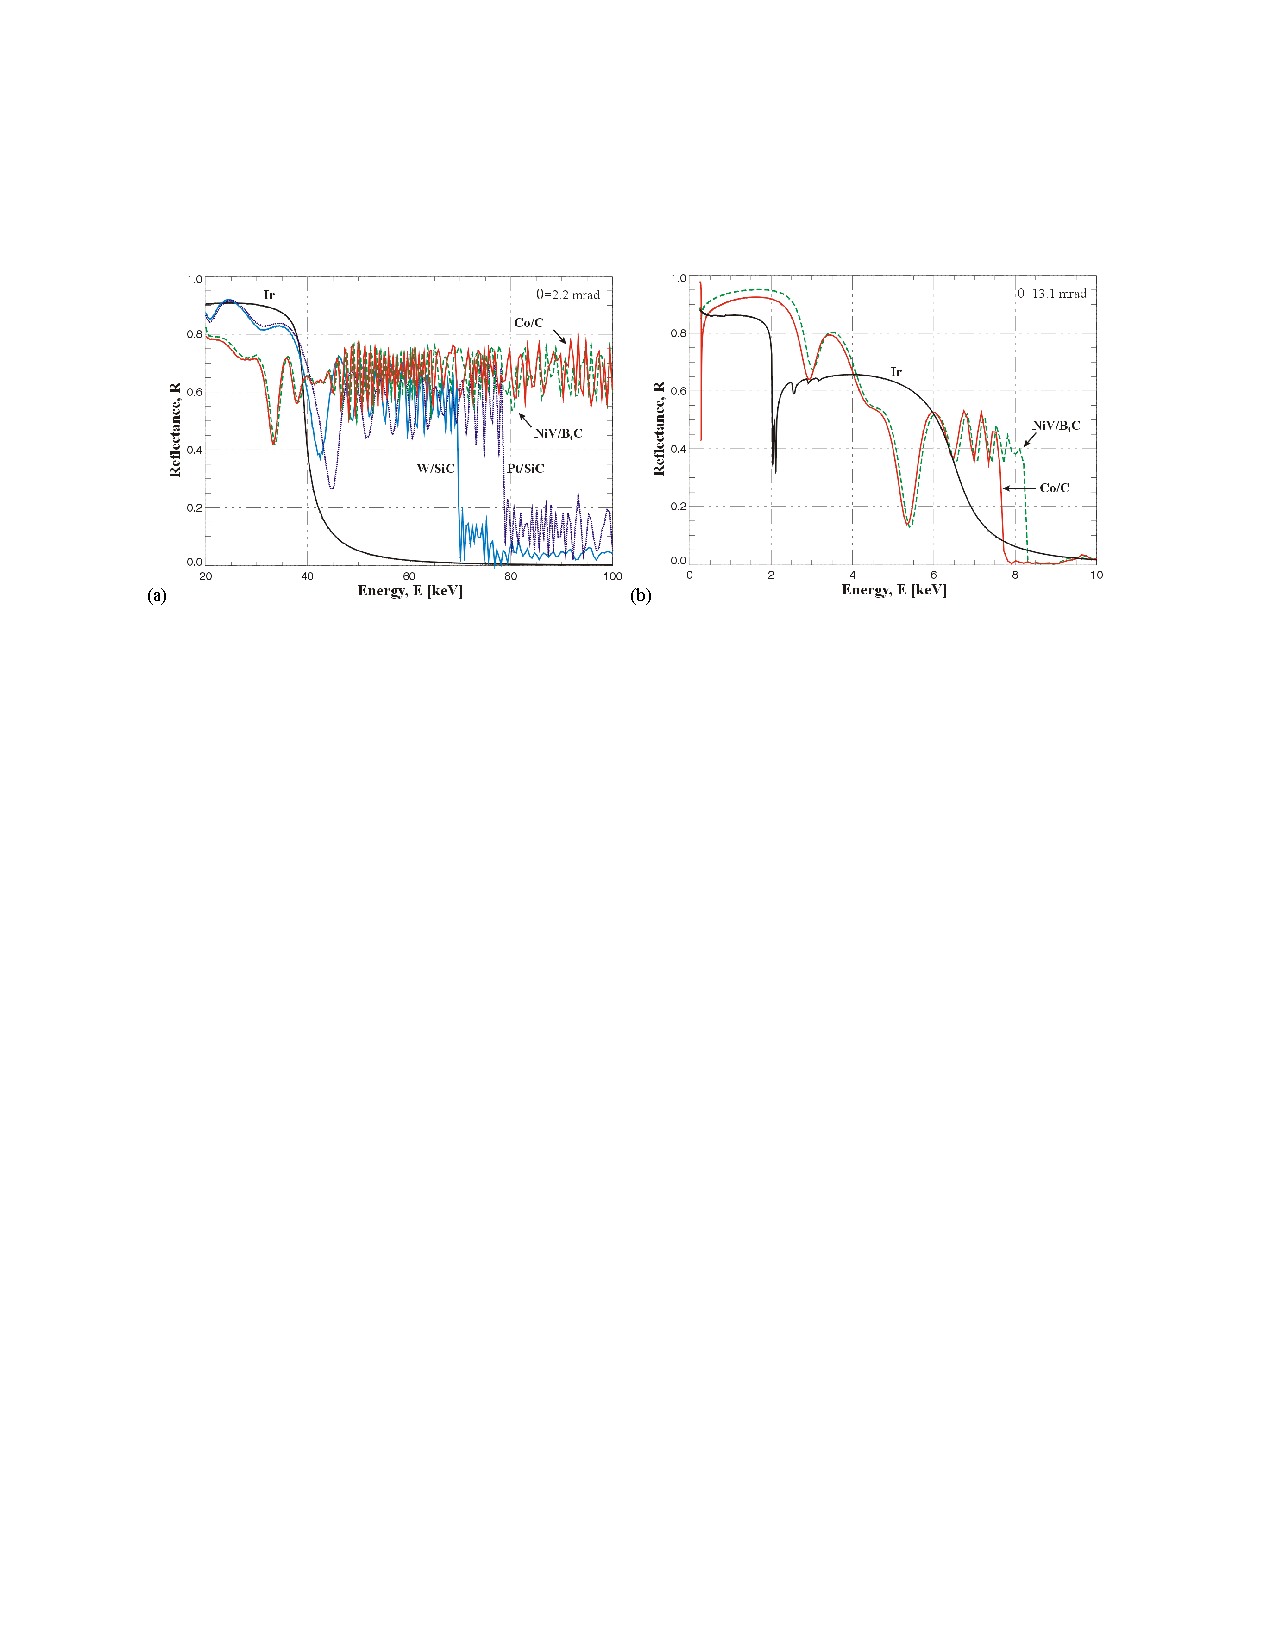
\includegraphics[width=\linewidth]{figures/introduction/xrayperformance.pdf}
	\caption{\footnotesize XRR simulations of an Ir singlelayer and a selection of multilayers as a function of energy. \textbf{(a)} shows the reflectivity response in range from 20 to 100 keV at a constant $2.2\text{mrad} = 0.126$\degr\ reflection angle. The Ir singlelayer loses nearly all reflectance around $40$ keV. W/SiC and Pt/SiC has drops around the absorption edges of W and Pt $69.5$ keV and $78.4$ keV. The reflectivity response from Co/C and NiV/B$_4$C is nearly constant in the entire spectrum. \textbf{(b)} shows the reflectivity response in the 0 to $10$ keV range at a constant angle of $13.1 \text{mrad} = 0.751$\degr. The Ir singlelayer loses reflectivity around $\sim 6.5$ keV, the Co/C multilayer at $\sim$7.6 keV and the NiV/B$_4$C at $\sim 8.3 $ keV. From \cite{Bellotti:2009dj}.}
	\label{fig:xrayperformance}
\end{figure}

To focus higher energies, it is necessary to use multilayers with bilayers of two different materials. These improve the performance significantly at higher energies as can be seen in figure \ref{fig:xrayperformance}(a). The two materials have to be one of high electron density (high Z) and one of low electron density (low Z), since it is the interfaces between two materials with high difference in refractive index that reflects the X-ray photons. The basic parameters that define a multilayer is:

\begin{itemize}
	\item[$\bullet$] $N$, the number of bilayers in the multilayer
	\item[$\bullet$] $d$, the thickness of the bilayers, also called the d-spacing
	\item[$\bullet$] $\Gamma$, the thickness ratio of low Z versus high Z materials
\end{itemize}

The multilayer can have a constant d-spacing through the entire stack and will then exhibit Bragg reflections as the interfaces will act like periodic lattice planes in a crystal. The Bragg condition ensures that only a certain energy can be reflected at a certain angle because of constructive interference. Other energies will not experience constructive interference, so the reflected intensity is neglible. When focusing non-monochromatic X-ray photons, but rather photons with a range of energies, it is necessary to have a mirror with a smooth energy response. To achieve that, the d-spacing can be changed through the stack according to a linear grading or a power-law grading\cite{Joensen:12je}, $d_i = a/(b+i)^c$, where $d_i$ is the d-spacing for the i'th layer. The constants are determined for values of $c$, $d_{min}$, $d_{max}$. The resulting so-called \emph{depth graded} multilayer have a smoother response curve, so are more suitable for astronomincal telescopes.

The material chosen as low Z and high Z materials will perform best if the difference in electron density is as large as possible. But there are other factors to consider: as can be seen in figure \ref{fig:xrayperformance}(a) W/SiC and Pt/SiC have a cut-off at 69.5 keV and 78.4 keV respectively. That is caused by X-ray absorption edges in W and Pt, which increases the absorption in the multilayer to a point where roughness decreases significantly.

Another factor to consider is the ability of the combination of two materials in a multilayer (e.g. W and SiC) to achieve low roughness in the interfaces between each layer. The interface between two layers can be described by an interface profile developed by Stearns et al\cite{Stearns:1989va}. The profile width is $\theta_{\text{rms}}=(\theta_r^2 + \theta_f^2)^{1/2}$, where $\theta_r$ is the roughness and $\theta_f$ is the diffuseness of the two materials in the interface. A general rule of thumb is to keep $\sigma_{rms} \leq d/6$, with $d$ being the thickness of a single bilayer. That means that a bilayer which is 3 nm thick can only have an average roughness of 0.5 nm, which is only the height of a few atomic monolayers. A roughness higher than that will cause loss of definition in the multilayer resulting in less defined Bragg peaks given by loss of reflectivity at the interfaces.

\subsection{NuSTAR}\label{sec:nustar}
\emph{This thesis has a number of references to the NuSTAR mission, so a short overview is given here.}

The NuSTAR telescope was the first mission to carry a hard X-ray (5-80 keV) focusing telescope to orbit, and the first in-orbit X-ray telescope to use graded-d multilayer coatings. It is a NASA mission made in collaboration between mainly Caltech, Columbia University, Lawrence Livermore National Lab., and DTU Space and was launched in 2012. Using an extendable mast, the focal length becomes 10 m when deployed in orbit.

\begin{figure}[!ht] % xrayperformance
	\centering	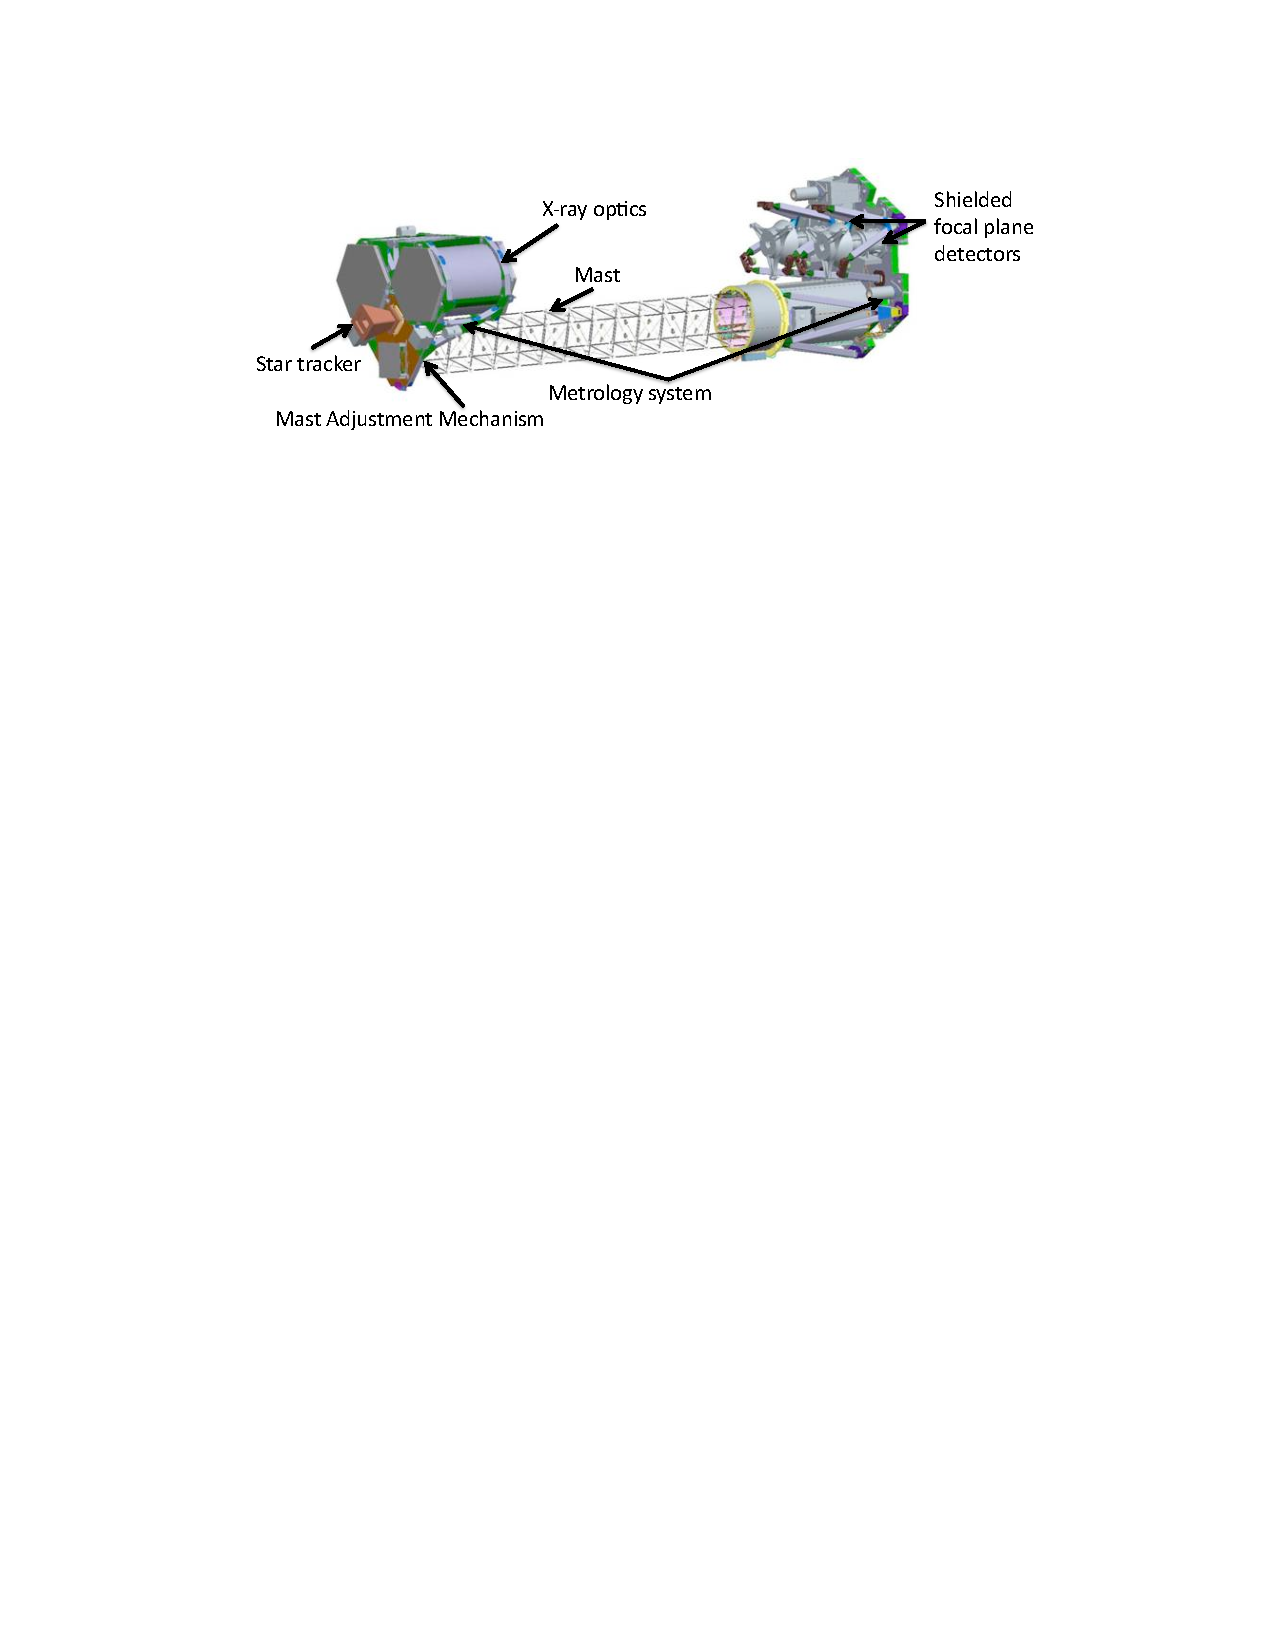
\includegraphics[width=0.8\linewidth]{figures/introduction/nustar.pdf}
	\caption{\footnotesize Diagram of the NuSTAR telescope with the extendable mast partially collapsed. From \cite{Harrison:2010gu}.}
	\label{fig:xrayperformance}
\end{figure}

It carries two Wolter I type telescopes that are made by rectangular pieces of 0.21 mm thick glass that is slumped to the curvature of each radius in the telescope\cite{Craig:2000fd,Hailey:1997ie}. The glass has a 0.4--0.5 nm r.m.s. roughness.

Each telescope consists of 133 concentric mirror shells of glass, with each glass substrate being 225 mm long. Two stacks of 133 shell layers fit together to make the first and second reflection of the Wolter I principle. The innermost and outermost shells have radii of 54.4 mm and 191 mm, respectively, making the total diameter of each telescope $\sim$400 mm. Glass substrates were mounted using graphite spacers that were machined to $\sim$2.5 $\upmu$m precision.

All glass substrates for NuSTAR were coated at DTU Space using multilayer material combinations of either W/Si or Pt/C. Multilayers of W/Si were 291 bilayers and multilayers of Pt/C were 145 bilayers. The multilayers were graded according to a power-law\cite{Christensen:1992uc}.
